\chapter{功能验证}
本章节主要基于上一章的电路图设计进行功能验证,用到的主要工具软件为NC。
\section{NC简介}
NC-Verilog是Candence公司的Verilog数字逻辑模拟器,具有运行快、精度高、调试功能强大、使用灵活等优点,是业界公认的黄金模拟器。NC-Verilog的运行分为两个步骤,首先是编译,检查语法错误等,然后模拟执行。NC-Verilog使用NCC技术,提高了模拟的性能减少了内存的使用。采用INCA架构,具备了支持多种HDL语言、多设计层次、数模混合设计的能力。

运行流程包括:建立列表文件,列表文件包含激励信号;建立配置文件,以一个脚本的形式对NC进行配置,包括启动GUI界面、开启覆盖率统计、访问权限等设置;运行NC-Verilog,以上一步的配置启动NC;波形查看与调试,可以通过“shm\_open”和“shm\_probe”两个命令来保存波形,并且可以查看信号的波形以及逻辑结构图等,这一步主要通过查看波形以确定模块的正确性;查看覆盖率,这一步同样需要一个TCL脚本文件进行配置,并借助ICCR软件进行分析;导出VCD文件,可以通过tcl脚本或NC软件或“dumpfile”“dumpvars”来完成。以上就是功能验证部分的工作流程。 
\section{NC验证结果}
由于存在多个模块需要验证,为方便操作,在完成“或”模块的功能验证后,借助如下所示脚本来准备下一模块功能验证所需的文件以及部分内容等。

\lstinputlisting[language=sh,basicstyle=\footnotesize\ttfamily,caption={准备NC所需的文件脚本},label=list3.1]{chapter2/prefile.sh}
其中\verb|head -n 5 ./OR2/OR2_tb.v > $1/$1_tb.v|为准备各个子模块公用的Testbench信息,共5行,具体内容如下:
{
\footnotesize
\begin{verbatim}
`timescale 10ns/1ns
module cds_globals;
supply1 VDD_;
supply0 GND_;
endmodule
\end{verbatim}
}
\noindent Testbench剩下的内容即为根据具体模块的实例化以及激励的产生等。

图\ref{fig3.1}所示为基本单元的功能验证波形。
\begin{figure}[!hbtp]
\centering
\subfigure[二输入与的验证结果]{
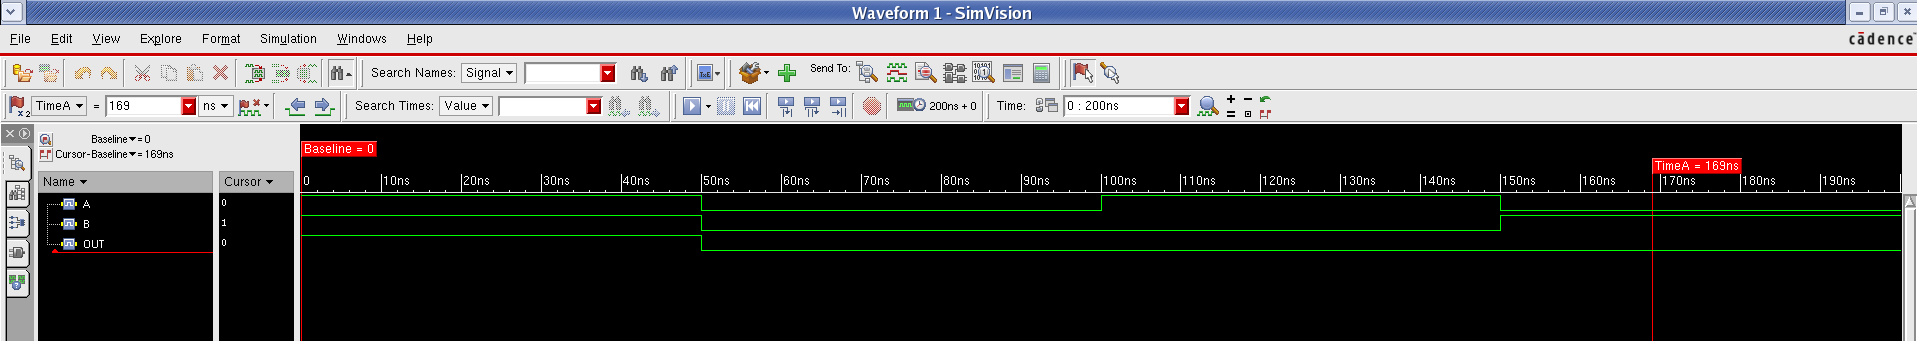
\includegraphics[width=0.9\textwidth]{chapter3/AND2_nc}
\label{fig3.1a}
}
\subfigure[三输入与或的验证结果]{
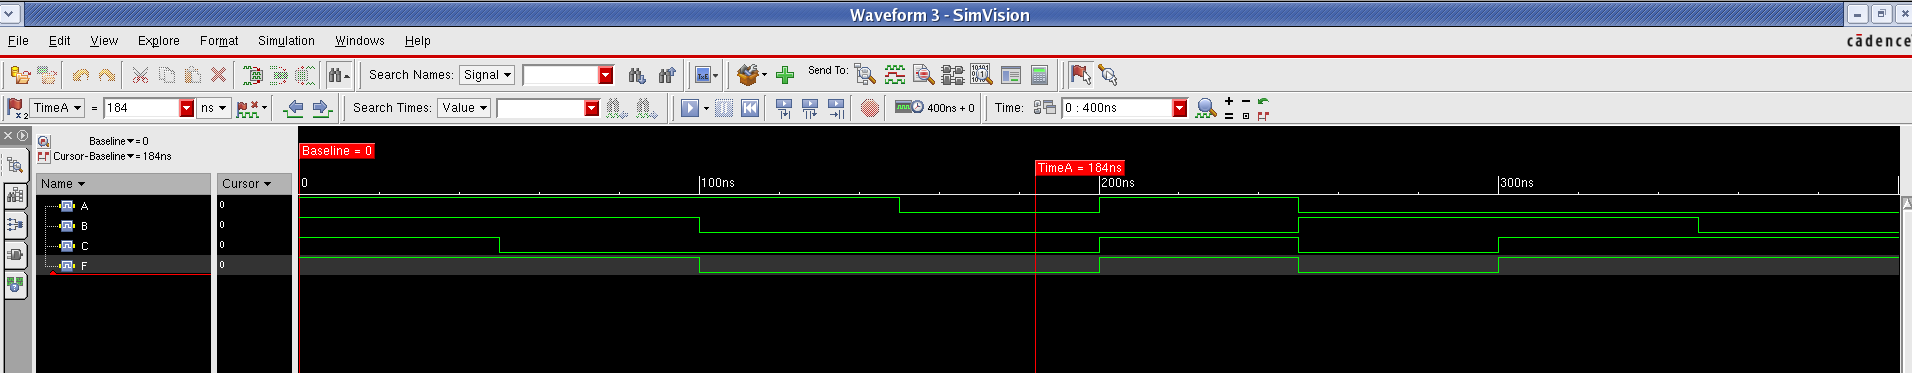
\includegraphics[width=0.9\textwidth]{chapter3/IAO_nc}
\label{fig3.1b}
}
\subfigure[两路31位选择器]{
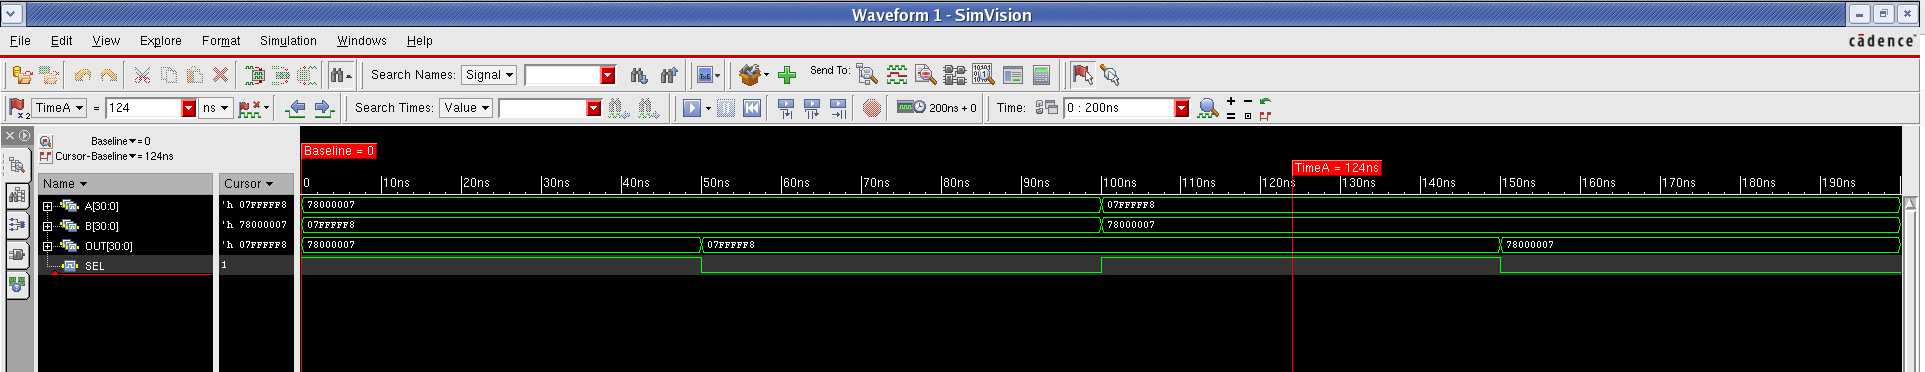
\includegraphics[width=0.9\textwidth]{chapter3/MUX2_31_nc}
\label{fig3.1c}
}
\caption{基本单元的NC验证结果}
\label{fig3.1}
\end{figure}\\
\indent 图\ref{fig3.2}所示为各级LZC模块的功能验证波形。
\begin{figure}[!hbtp]
\centering
\subfigure[4-bit LZC验证结果]{
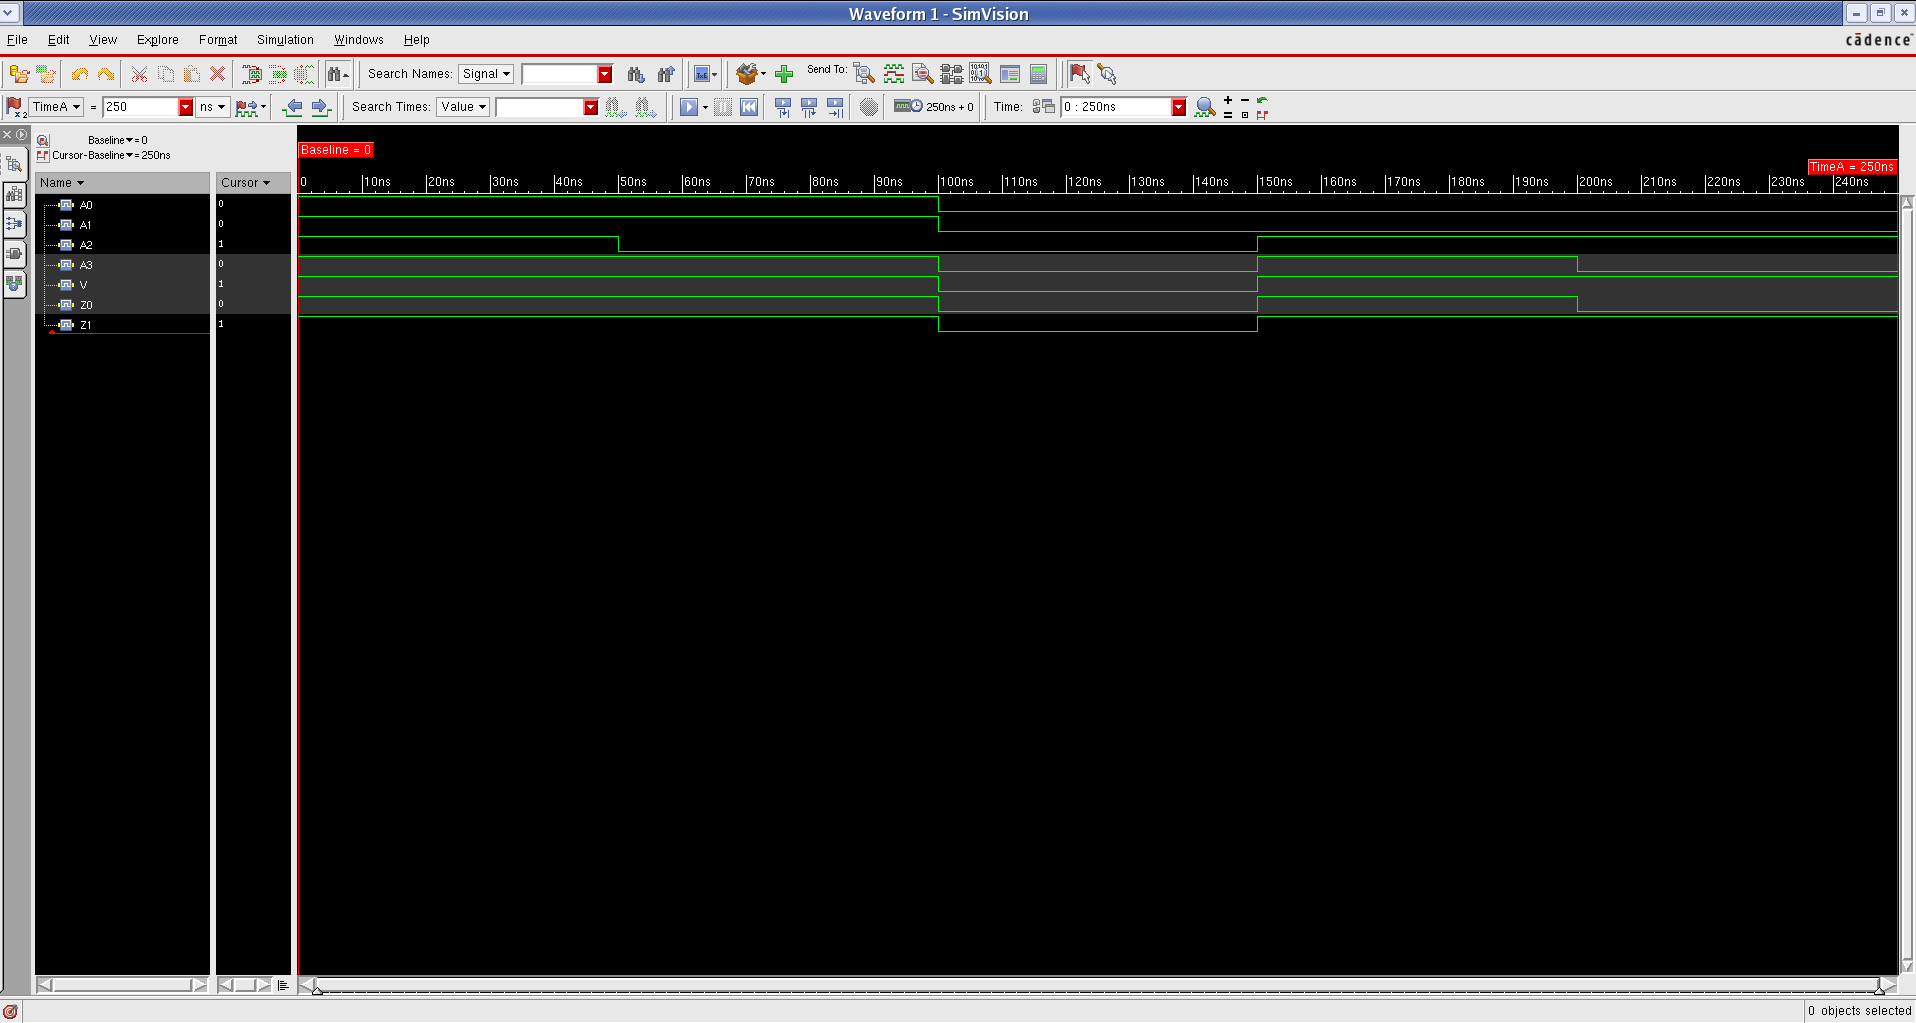
\includegraphics[width=0.9\textwidth]{chapter3/LZD4_nc}
\label{fig3.2a}
}
\subfigure[16-bit LZC验证结果]{
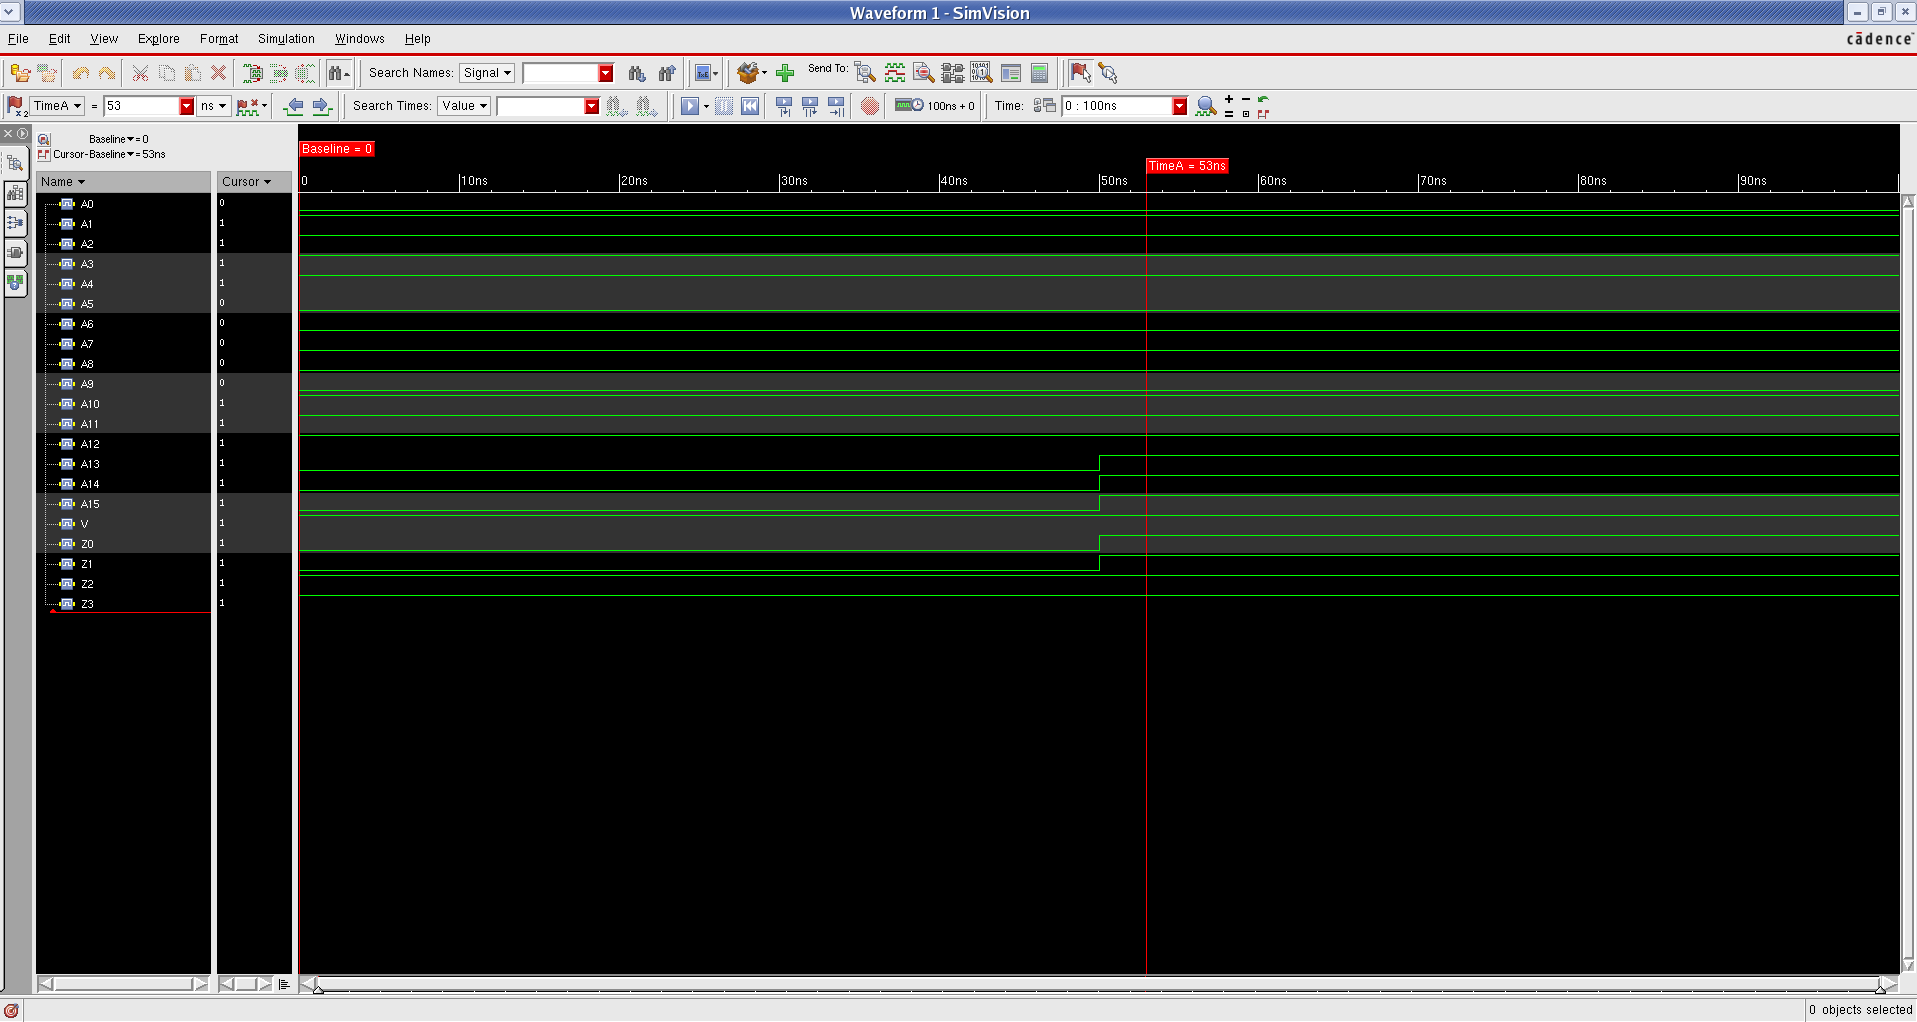
\includegraphics[width=0.9\textwidth]{chapter3/LZD16_nc}
\label{fig3.2b}
}
\caption{LZC单元的NC验证结果}
\label{fig3.2}
\end{figure}\\
\indent 最后,基于图\ref{fig2.3}所示的NORM指令的NC验证结果如图\ref{fig3.3}所示。表\ref{table3.1} 给出了LZC模块以及NORM指令模块的输入与输出的关系,其中LZC模块的输出为真实值的相反数,且在输入数的所有位全为0的时候,$V$也为0(实际值为1)。{\bfseries 从表\ref{table3.1}可以看出,图\ref{fig2.3}所示的NORM电路图可以正确的实现NORM指令的功能,即统计符号位后与符号位相同值的连续位数。}
\begin{table}[!hbpt]
\centering
\caption{LZC模块以及NORM模块的NC验证结果}
\label{table3.1}
\begin{tabular}{ccc}
\toprule
模块   & 输入   & 输出   \\
\midrule
\multirow{3}{*}{4-bit LZC} & 0100 & 10 \\
 & 1011 & 11 \\
 & 0000 & 00($V=0$) \\
\multirow{2}{*}{16-bit LZC} & 16'h1C1E & 1100  \\
& 16'hFC00 & 1111\\
\multirow{5}{*}{NORM模块} & 32'h0000\_FFFF& 32'h0000\_000F \\
& 32'hFFFF\_0000 & 32'h0000\_000F \\
& 32'h0F00\_0000 & 32'h0000\_0003 \\
& 32'h00F0\_0000 & 32'h0000\_0007 \\
& 32'hFF0F\_0000 & 32'h0000\_0007 \\

\bottomrule
\end{tabular}
\end{table}

对于NORM指令模块,输入(Src)为$32'hFFFF\_0000$和$32'h0000\_FFFF$时,输出(Lzc)是相同的,均为$32'h0000\_000F$,由于NORM指令的统计过程并不包括符号位在内,因此最终的结果为15而不是16,同理,输入为其它数值时也有类似结果。
\begin{figure}[!hbtp]
\centering
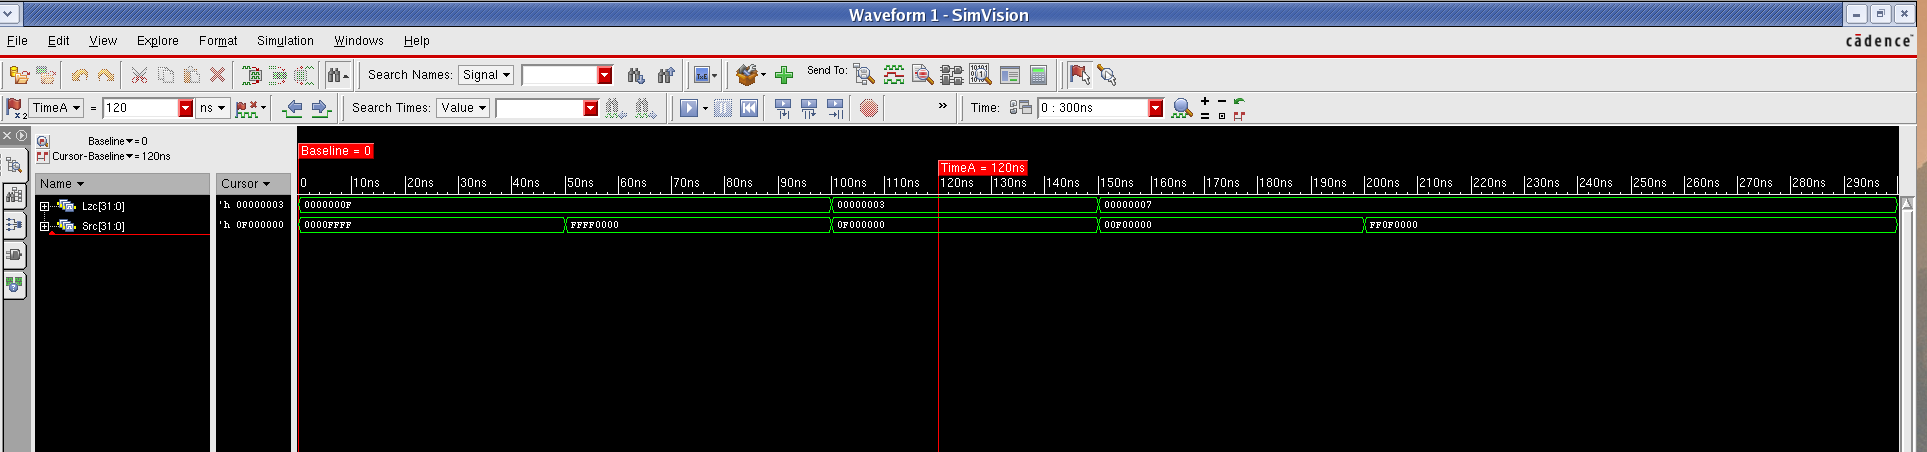
\includegraphics[width=0.9\textwidth]{chapter3/NORM_nc}
\caption{NORM模块NC验证结果}
\label{fig3.3}
\end{figure}